\documentclass[10pt,a4paper,titlepage]{report}
\usepackage[latin1]{inputenc}
\usepackage{amsmath}
\usepackage{amsfonts}
\usepackage{amssymb}
\usepackage[labelfont=bf]{caption}
\usepackage{float}
\usepackage[section]{placeins}
\usepackage{graphicx}
\usepackage[left=2cm,right=2cm,top=2cm,bottom=2cm]{geometry}
\author{Elijah Andrews}
\title{Implementing the Discrete Element Method with OpenCL for GPUs}
\begin{document}
\tableofcontents
\chapter{Introduction}
\section{Previous Work}
\section{Project Goals}
\chapter{The Discrete Element Method}
\section{Forces}
\section{Collision Detection}
\section{Implicit/Explicit}
\section{Rotation/Quaternions}
\chapter{OpenCL and Graphics Processing Units}
\chapter{Python Implementation}
\section{Overview}
\section{Element Types}
\subsection{Particle}
\subsection{Axis-Aligned Simple Wall}
\section{Collision Detection}
\section{Calculating Forces}
\subsection{Drag}
\subsection{Gravity}
\subsection{DEM Forces}
\section{Numerical Integration}
\subsection{Velocity}
\subsection{Position}
\subsection{Method of Integrating Drag}
There are three different methods of integrating drag. Firstly, there is the analytical solution, this is the exact solution to the model but cannot be done easily computationally. Secondly, there is the explicit numerical solution, this takes the current state and estimates the future state. Thirdly, there is the implicit numerical solution, this assumes the future state and integrates accordingly.
For a simple system with constant flow speed and no gravity, the system acceleration is described by equation \ref{eq:drag_acceleration}.
\begin{equation}
\dot{u} = \dfrac{v-u}{\tau}
\label{eq:drag_acceleration}
\end{equation}
Equation \ref{eq:drag_acceleration} can be solved to show that the analytical solution for the particle speed, $u$, is that in equation \ref{eq:analytical_drag_speed}.
\begin{equation}
u(t) = v(1 - e^{-\dfrac{t}{\tau}})
\label{eq:analytical_drag_speed}
\end{equation}
The explicit numerical integration method for equation \ref{eq:drag_acceleration} is that in equation \ref{eq:explicit_drag_speed}. Where $u_{n}$ is the current speed and $u_{n+1}$ is the speed after timestep $\Delta t$.
\begin{equation}
\dfrac{u_{n+1} - u_{n}}{\Delta t} = \dfrac{v - u_{n}}{\tau}
\label{eq:explicit_drag_speed}
\end{equation}
The implicit numerical integration method for equation \ref{eq:drag_acceleration} is that in equation \ref{eq:implicit_drag_speed}. Where $u_{n}$ is the current speed and $u_{n+1}$ is the speed after timestep $\Delta t$.
\begin{equation}
\dot{u} = \dfrac{u_{n+1} - u_{n}}{\Delta t} = \dfrac{v - u_{n+1}}{\tau}
\label{eq:implicit_drag_speed}
\end{equation}
Equation \ref{eq:implicit_drag_speed} can be rearranged to get an equation of the form $\dot{u} = f(u_{n})$ as shown in equation \ref{eq:implicit_drag_acceleration}.
\begin{equation}
\dot{u} = \dfrac{v - u_{n}}{\tau + \Delta t}
\label{eq:implicit_drag_acceleration}
\end{equation}
When these three methods are applied to the system they produce the results in figure \ref{fig:particle_speed_for_different_integrations}.
\begin{figure}[h!]
\centering
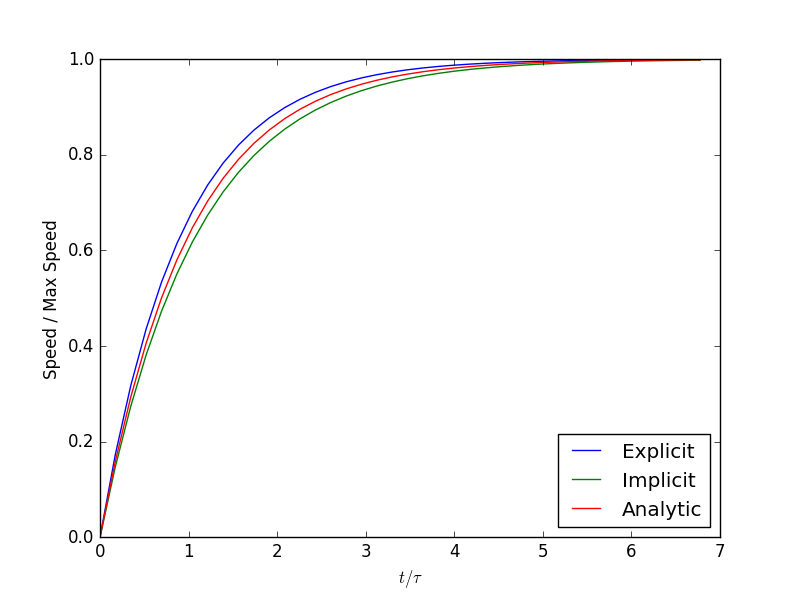
\includegraphics[scale=0.75]{figures/ParticleSpeedWithVaryingIntegration.png}
\caption{A graph of particle speed against time for the three methods of integration.}
\label{fig:particle_speed_for_different_integrations}
\end{figure}
\\Comparing the explicit and implicit numerical integration to the analytical solution shows that the explicit method has an average percentage difference of 2.05\% and the implicit method has an average percentage difference of 1.85\% when the timestep is $0.1 s$.
\\The average percentage difference can be compared between the two methods with varying timesteps as shown in figure \ref{fig:avg_percent_diff_against_timestep}. This graph shows that the explicit method increases its average percentage difference approximately linearly with increasing timestep. The implicit method increases its average percentage difference non-linearly at a slower rate than the explicit method. This implies that the implicit method is more accurate than the explicit method, especially for higher timesteps.
\begin{figure}[!htb]
\centering
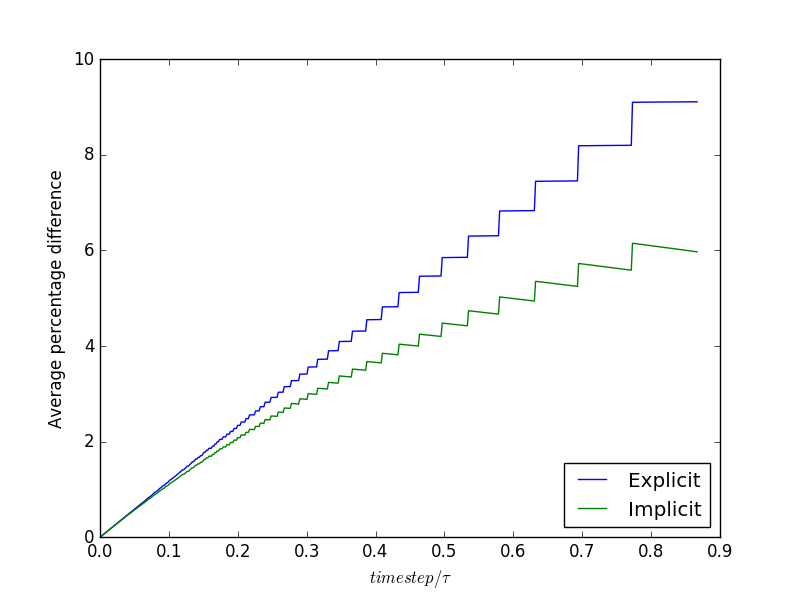
\includegraphics[scale=0.75]{figures/AveragePercentageDifferenceAgainstTimestep.png}
\caption{A graph of average percentage difference between the numerical method and analytical solution against varying timestep.}
\label{fig:avg_percent_diff_against_timestep}
\end{figure}
\\Unlike the explicit method, the implicit method depends on the other accelerations in the system. Equation \ref{eq:implicit_drag_acceleration} can be redefined to include these other accelerations as an extra $\dot{u}_{e}$ term as shown in equation \ref{eq:drag_acceleration_with_other_accelerations}.
\begin{equation}
\dot{u} = \dfrac{u_{n+1} - u_{n}}{\Delta t} = \dfrac{v - u_{n+1}}{\tau} + \dot{u}_{e}
\label{eq:drag_acceleration_with_other_accelerations}
\end{equation}
As before, equation \ref{eq:drag_acceleration_with_other_accelerations} can be rearranged to be in the form $\dot{u} = f(u_{n})$ as shown in equation \ref{eq:implicit_drag_acceleration_with_other_accelerations}.
\begin{equation}
\dot{u} = \dfrac{v - u_{n} + \tau \dot{u}_{e}}{\tau + \Delta t}
\label{eq:implicit_drag_acceleration_with_other_accelerations}
\end{equation}
Equation \ref{eq:implicit_drag_acceleration_with_other_accelerations} can be applied to a particle falling under the effect of gravity through a stationary fluid. The results are shown in figure \ref{fig:fig:terminal_velocity_implicit_explicit}. As with the previous system, the explicit method has an average percentage difference of 2.05\% and the implicit method has an average percentage difference of 1.85\% when the timestep is $0.1 s$. This shows that the accuracy of the modified equation is consistent with that of equation \ref{eq:implicit_drag_acceleration}.
\begin{figure}[!htb]
\centering
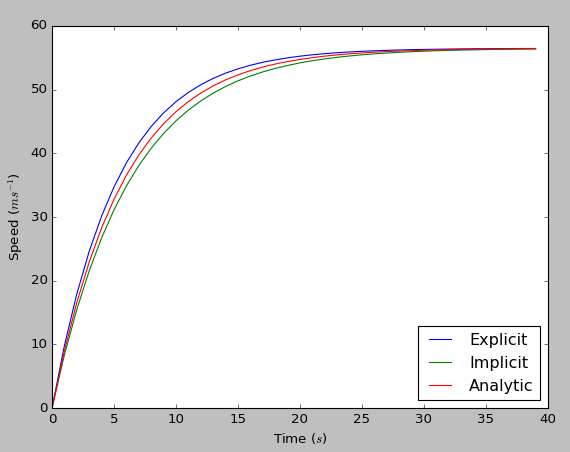
\includegraphics[scale=0.75]{figures/TerminalVelocityImplicitExplicit.png}
\caption{A graph of particle speed against time for each method of integration using equation \ref{eq:implicit_drag_acceleration_with_other_accelerations}.}
\label{fig:fig:terminal_velocity_implicit_explicit}
\end{figure}
\section{Verification (accuracy?)}
To asses the accuracy of the implementation a series of cases have been tested and compared to analytical solutions of the model.
\subsection{Settling Overlap}
In this case two particles are used. The first particle is an ordinary particle acting under the effects of gravity. The second particle, placed below the first particle, is a particle with quasi-infinite density without being affected by gravity. As time increases the first particle bounces on the second particle until it eventually comes to rest with some overlap with the second particle.\\
\begin{figure}[!htb]
\centering
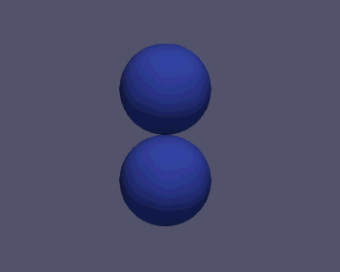
\includegraphics[scale=0.75]{figures/ParticleRestingOnOtherParticle.png}
\caption{A particle, under the effect of gravity, resting upon a second particle of infinite density, unaffected by gravity.}
\end{figure}
\\For the particle to be at rest the particle's gravity must be equal to the normal force from the DEM.
\begin{equation}
F_{g} = F_{n}
\end{equation}
\begin{equation}
mg = k_{e}\delta - \eta u
\end{equation}
To get an equation for overlap, $\delta$, the equation is simplified and rearranged. The speed, $u$, is 0 at rest.
\begin{equation}
\delta = \dfrac{mg}{k_{e}}
\end{equation} 
Taking particle diameter to be 0.1 $m$ and particle density to be 2000 $kg m^{-3}$, the particle mass is 1.047 $kg$. Gravity is taken to be 9.81 $m s^{-2}$ and model spring stiffness is $10^{5}$.
\begin{equation}
\delta = \dfrac{1.047 * 9.81}{10^{5}} = 1.027 * 10^{-4}
\end{equation} 
Running a simulation with these parameters also yields an overlap of $1.027 * 10^{-4}$. Comparing simulation results with high precision overlap prediction shows that the simulation result is within $2.1 * 10^{-11}\%$ of the predicted value.
\subsubsection{Timestep stability}
This result can also be compared for varying timesteps to asses the stability of the implementation. Figure \ref{fig:overlap_percentage_error_against_timestep} shows very stable results up until a timestep of approximately 0.00097.
\begin{figure}[!htb]
\centering
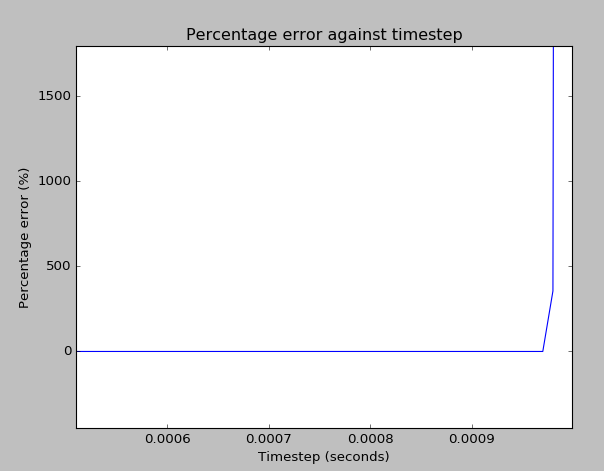
\includegraphics[scale=0.75]{figures/ParticleBounceTimestepAgainstPercentageError.png}
\caption{A graph of overlap percentage error against time step.}
\label{fig:overlap_percentage_error_against_timestep}
\end{figure}
\subsection{Terminal Velocity}
As mentioned in [ref], integrate and compare with different timesteps.
\subsection{Timestep Stability}
Collisions go boom if timestep is too high etc. <Test against bouncing or something>
This can be spotted and logged if $E_{k}$ is higher after collision than before.
\chapter{OpenCL Implementation}
\chapter{Results}
\section{Comparison between CPU and GPU}
\chapter{Conclusion}
\section{Further Work}
\end{document}
